\section{Anti-aliasing}
\begin{center}
    Конспект составила: \textit{Александра Лановая}
\end{center}

\subsection{Aliasing}
Если частота дискретизации слишком низкая, возникает проблема, известная как aliasing. Это явление проявляется, когда мы преобразуем аналоговый сигнал в цифровой, но частота выборок оказывается недостаточной. Представьте, что мы хотим оцифровать синусоидальную волну и начинаем сэмплировать её точки с недостаточной частотой. Соединив полученные точки, мы обнаружим, что восстановленный сигнал отличается от исходного. Это приводит к тому, что цифровая волна имеет другую частоту, чем аналоговая. Когда происходит aliasing, восстановить исходный сигнал невозможно. Чтобы избежать этого, необходимо изначально записывать данные с более высокой частотой дискретизации.

\begin{figure}[H]
    \centering
    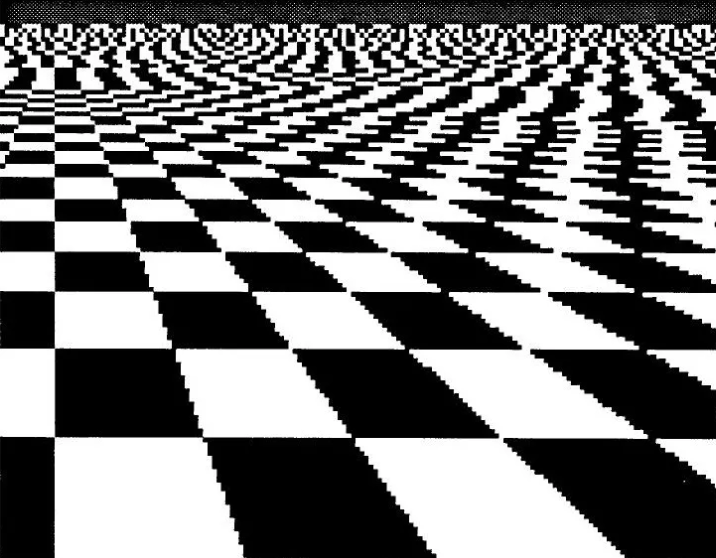
\includegraphics[width = 6cm]{1.png}
    \caption{Пример aliasing}
    \label{fig:float}
\end{figure}

\textbf{Aliasing }— это артефакт, возникающий из-за неправильной частоты дискретизации. Существует правильная частота (Найквиста-Шеннона), но её использование требует дополнительных вычислений.

В графике aliasing выражается в эффекте <<зубчатости>> границ на изображении или как муаровый узор. Чтобы избавиться от aliasing'а, необходимо применять корректную пространственную выборку. Однако это требует перехода от изображения к частотному домену с использованием прямого и обратного преобразования Фурье, что очень ресурсоёмко. поэтому были разработаны менее требовательные к вычислениям приближения.

Aliasing проявляется по-разному в зависимости от контекста:

\begin{itemize}
    \item \textbf{Геометрический алиасинг:} выражается в виде ступенчатости пикселей на краях объектов.
    \item \textbf{Подпиксельный алиасинг:} возникает, когда узкие объекты, например линии электропередач, исчезают на больших расстояниях.
    \item \textbf{Aliasing прозрачности:} проявляется при отображении множества мелких объектов, например листвы деревьев, которая начинает <<мерцать>> при удалении.
\end{itemize}

Алгоритмов решения проблемы было придумано очень много разными компаниями в разные года, некоторые являются частными случаями других, некоторые являются логическим продолжением других, мы рассмотрим только часть из них, которые сильно отличаются концептуально.
\subsection{Super Sampling Anti-Aliasing, SSAA}

Это самый старый и самый простой метод сглаживания. Он включает в себя рендеринг сцены с более высоким разрешением, чем заданная настройка, а затем сэмплинг и смешивание результата до меньшего числа пикселей. Например, монитор может быть иметь разрешение 1920x1080 пикселей, а игру можно настроить для рендеринга с разрешением 3840x2160, после чего происходит масштабирование обратно до меньшего разрешения и вывод результата на экран. Обычно в этом алгоритме используется метод ближайшего соседа, а математика смешивания является ни чем иным, как средним арифметическим сэмплов.

Поскольку сами пиксели имеют дискретную область, позиции сэмплов могут быть установлены в любом месте в пределах этой области. Хотя количество способов, которыми это можно сделать, бесконечно, есть несколько способов, которые обычно используются:

\begin{itemize}
    \item \textbf{Сетка:} это самый простой алгоритм. Пиксель разбивается на несколько субпикселей, и выборка берется из центра каждого. Этот метод быстро реализуется, но из-за регулярной природы выборки алиасинг все еще может возникать, если используется небольшое количество субпикселей.
    \item \textbf{Рандом:} этот метод избегает регулярности выборки сетки. Однако из-за нерегулярности шаблона выборки могут оказаться ненужными в некоторых областях пикселя и отсутствовать в других.
    \item \textbf{Шум Пуассона:} алгоритм выборки шума Пуассона размещает сэмплы случайным образом, но затем проверяет, чтобы любые два сэмпла не находились слишком близко друг к другу. В результате получается равномерное, но случайное распределение сэмплов. Наивный алгоритм «метания дротиков» был очень медленным для больших наборов данных, что ограничивало его применение в рендеринге в реальном времени. Однако сейчас существует множество быстрых алгоритмов для генерации шума диска Пуассона, даже с переменной плотностью.

    \item \textbf{Джиттер:} это модификация алгоритма сетки, при которой пиксель разбивается на несколько субпикселей, но выборка берется не из центра каждого, а из случайной точки внутри субпикселя.
    \item \textbf{Повернутая сетка:} этот метод использует сетку $2\times2$, но шаблон сэмпла поворачивается, чтобы избежать выравнивания сэмплов по горизонтальной или вертикальной оси. Это значительно улучшает качество сглаживания для наиболее часто встречающихся случаев. Для оптимального шаблона угол поворота равен $arctan(1/2)$ (примерно 26,6 градуса), и квадрат растягивается в $\sqrt{5/2}$. Интересно, что эта задача напоминает задачу о том, как разместить 8 ферзей на шахматной доске $8\times8$ так, чтобы никакие два ферзя не угрожали друг другу.
\end{itemize}

Эти паттерны и образуют различные алгоритмы суперсэмплинга. Суперсэмплинг позволяет добиться очень качественного изображения, которое приятно глазу во многих случаях по сравнению с другими алгоритмами. Кроме того, сам алгоритм достаточно прост в реализации.

На сегодняшний день суперсэмплинг используется реже, хотя нашел новое применение в качестве настроек в драйверах для видеокарт AMD и NVIDIA. В AMD эта технология называется виртуальное суперразрешение (Virtual Super Resolution, VSR), а в NVIDIA — динамическое суперразрешение (Dynamic Super Resolution, DSR). Эти технологии можно использовать для сглаживания в некоторых старых играх, в которых нет встроенной системы сглаживания, или просто для улучшения уже имеющегося изображения.

Однако у суперсэмплинга есть свои недостатки. Все дополнительные пиксели необходимо обрабатывать, и увеличение разрешения может легко привести к резкому падению частоты кадров (FPS). Даже с учетом того, что видеокарта уже умеет быстро менять разрешение картинки, нам все равно нужно обрабатывать каждый пиксель на картинке большего разрешения, чтобы сформировать итоговый цвет.

В связи с этим был разработан адаптивный алгоритм суперсэмплинга, который предлагает более эффективное решение. Самое простое решение заключается в том, чтобы обрабатывать только края объектов. Это позволяет значительно сократить количество пикселей, которые необходимо обрабатывать, и, как следствие, улучшить производительность без значительной потери качества изображения.

\subsection{Multi-Sampling Anti-Aliasing, MSAA}
Метод, о котором идет речь, впервые появился в исследовательских лабораториях Silicon Graphics в начале 90-х годов. По сути, это тот же суперсэмплинг (SSAA), но с выборочным применением только в тех местах, где это действительно необходимо. Но как же реализовать этот подход?

К счастью, необходимая информация для этого у нас уже есть. Когда трехмерный мир вершин преобразуется в двухмерную плоскость растра, в пикселях, образующих различные примитивы в сцене, закладывается информация не только о цвете и текстурах, но и о глубине. Эта информация может храниться в z-буфере (или буфере глубины), который затем используется для определения видимости краев.

\begin{figure}[H]
    \centering
    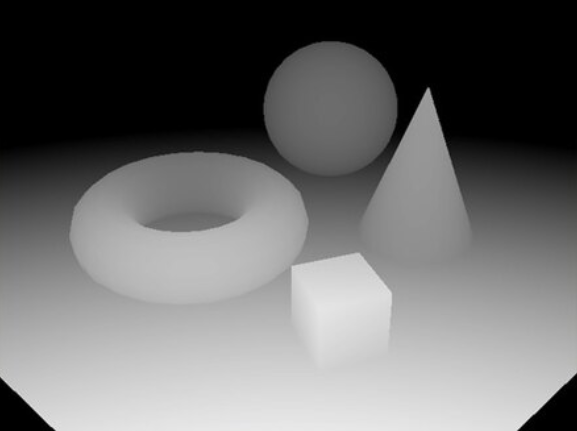
\includegraphics[width = 6cm]{7.png}
    \caption{Буфер глубины}
    \label{fig:float}
\end{figure}

Важно отметить, что шейдеры играют ключевую роль в этом процессе. Шейдеры — это программы, которые выполняют специализированные функции, такие как вычисление освещения и итоговых цветов объектов. Они напрямую работают с видеокартой, представляя собой абстракцию, которая указывает видеокарте, как нужно отрисовать объекты. Пиксельные шейдеры, также известные как фрагментные шейдеры, вычисляют цвет и другие атрибуты каждого <<фрагмента>> — единицы работы рендеринга, влияющей максимум на один выходной пиксель.

Мы можем создать версию черно-белой сетки с более высоким разрешением. В этом случае мы просто записываем глубину примитива в местах выборки. Отложив эту карту глубины, мы возвращаемся к кадру с исходным разрешением и запускаем все наши пиксельные шейдеры для формирования конечного цвета. Затем мы снова обращаемся к детализированному буферу глубины и для каждого пикселя, находящегося в примитиве (т.е. для черных пикселей), выделяем цвет шейдера на выходе. Очевидно, что это нужно где-то хранить, поэтому нам понадобится относительно небольшой буфер для каждой точки из выборки в пикселе. После этого, как и в случае с SSAA, мы сэмплируем и смешиваем детализированный буфер до требуемого разрешения, получая фрейм со сглаживанием. Что касается производительности, то мы запускаем пиксельные шейдеры только на относительно небольшом количестве точек, но при этом нам пришлось создать и сохранить пару буферов с высоким разрешением.

В отличие от SSAA, который улучшает все, метод MSAA (Multisample Anti-Aliasing) влияет только на края геометрии. Хотя это не представляет большой проблемы для статических изображений, в движении разница будет гораздо более заметной. Другая проблема заключается в том, что алгоритм плохо работает с отложенным рендерингом. Хотя существуют способы обойти это ограничение, ни один из них не будет <<бесплатным>> с точки зрения производительности. Отложенный рендеринг, если говорить грубо и коротко, — это техника, при которой отрисовка производится в несколько этапов: сначала рисуется геометрия, то есть позиция, нормали и материалы каждого объекта, а затем уже применяется освещение.

\subsection{Fast Approximate Anti-Aliasing, FXAA}
В 2009 году Nvidia представила новый метод очистки неровных краев фигур в 3D-сценах, известный как FXAA (Fast Approximate Anti-Aliasing). В отличие от SSAA и MSAA, реализация FXAA была разработана полностью при помощи шейдеров. С момента своего выпуска этот метод претерпел множество улучшений и сегодня активно используется в играх.

Алгоритм FXAA представляет собой проход постобработки, то есть запускается после того, как большая часть рендеринга уже завершена. Обычно он имеет вид однопиксельного шейдера. Первая итерация алгоритма работает следующим образом: сначала мы выбираем буфер, содержащий изображение, которое мы хотим отобразить, и преобразуем значение sRGB в линейную оценку яркости этого пикселя. Это мера того, сколько света проходит через заданную область в заданном направлении.

\begin{figure}[H]
    \centering
    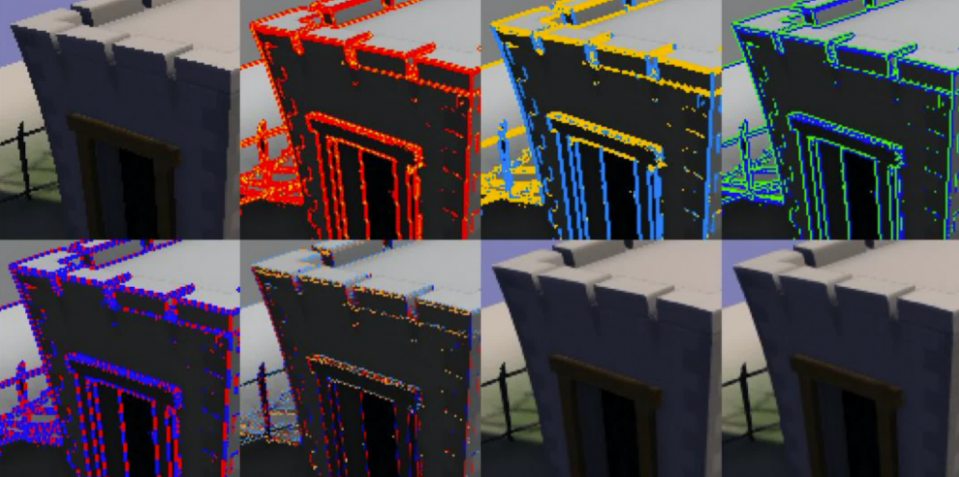
\includegraphics[width = 9cm]{8.png}
    \caption{Процесс выделения границ}
    \label{fig:float}
\end{figure}

Следующий шаг в шейдере включает проверку относительного контраста окружающих пикселей по отношению к выбранному пикселю. Если разница велика, это место, скорее всего, окажется границей. Отобранные пиксели проходят еще одну проверку для определения ориентации границы.

После идентификации всех краев на изображении позиции пикселей вдоль этих краев сдвигаются: вверх или вниз в случае горизонтальных линий, и из стороны в сторону для вертикальных линий. Перемещения происходят на небольшие расстояния, так что новое положение остается в пределах области исходного пикселя. Исходный буфер кадра дискретизируется с использованием новых местоположений: пиксели внутри примитивов по-прежнему остаются на своих местах, но те, что определяют границы, изменяются. Это помогает уменьшить влияние aliasing'а и делает края объектов более плавными и естественными.

Таким образом, FXAA представляет собой эффективный метод сглаживания, который позволяет улучшить качество изображения без значительного увеличения нагрузки на производительность. Он особенно полезен в играх и приложениях, где важна высокая частота кадров и плавность анимации. В отличие от более традиционных методов, таких как SSAA и MSAA, FXAA не требует рендеринга с высоким разрешением, что делает его более доступным для использования в реальном времени.

\subsection{Temporal Anti-Aliasing, TAA}
До сих пор мы рассматривали только методы борьбы с визуальным воздействием пространственного алиасинга. Однако для противодействия временному aliasing'у, который возникает из-за того, что 3D-игры генерируют дискретные выборки непрерывного движения, чаще всего используется следующий алгоритм.

Процесс рендеринга начинается как обычно, но затем значения цвета пикселей сохраняются в блоке памяти, называемом буфером истории. После этого рендеринг переходит к следующему кадру в последовательности и обрабатывает его. Перед отображением нового кадра мы берем сэмплы из буфера истории, и результат смешивается с текущим кадром. Затем буфер истории обновляется с новым результатом, копируется для формирования окончательного изображения, и в конце отмечается как готовый для отображения на мониторе.

Все последующие кадры следуют тому же шаблону рендеринга: сэмплируют буфер истории, смешивают, обновляют и отображают результат. Накопление последовательных кадров приводит к сглаживанию всей сцены при переходе от кадра к кадру, что создает гладкое изображение, на которое приятно смотреть.

Однако если бы работа алгоритма заканчивалась на этом, он был бы бесполезен. Например, если бы от кадра к кадру не было изменений, смешивание ничего не исправило бы. Чтобы обойти эту проблему, каждый кадр изначально рендерится со случайным смещением камеры с небольшим запасом, что называется субпиксельным дрожанием. Слегка сдвинутые позиции пикселей затем используются для сэмплирования буфера истории, после чего дрожание устраняется, и обработка кадра считается завершенной. Таким образом, когда дело доходит до смешивания значений истории с текущими, вы почти всегда получаете выборки координат субпикселей, которые находятся не совсем в одном и том же месте, что приводит к некоторой степени сглаживания.

Существует множество модификаций этого алгоритма, которые улучшают его работу. Например, есть эвристики верификации буфера истории, которые предотвращают использование значений из предыдущих кадров, которые больше не актуальны в текущем (например, если они скрыты за перемещенным объектом).

Тем не менее, временной антиалиасинг (TAA) может вызвать такую проблему, как гостинг (ghosting), когда края движущихся объектов кажутся размытыми, а не сглаженными. Чтобы избежать этого, используется шейдер для вычисления векторов движения объектов, сохранения информации в памяти (буфере скорости) и последующего сравнения относительных скоростей текущего пикселя с выбранными. Если они заметно отличаются, выборка истории отклоняется.

Для разработчиков запрограммировать все это гораздо сложнее, чем просто добавить в игру SSAA или MSAA. Однако современные графические процессоры могут довольно быстро обрабатывать все требуемые шейдеры. В то время как алгоритмы супер- и мультисэмплинга требуют множества сэмплов для каждого кадра (что увеличивает нагрузку на модуль вывода рендеринга (ROP) и пропускную способность памяти), TAA эффективно распределяет эти сэмплы по нескольким кадрам. Это означает, что для игр, не сильно ограниченных количеством затенения, можно включить TAA с относительно небольшой потерей производительности.

Кроме того, TAA хорошо работает с отложенным рендерингом и может использоваться в связке с FXAA и SMAA, что приводит к еще лучшему качеству изображения. К сожалению, он имеет склонность к чрезмерной размытости и может вызывать мерцающие артефакты на краях с высокой контрастностью.

\subsection{Другие алгоритмы}
Существует еще несколько алгоритмов, которые стоит упомянуть.

Первый из них —\textbf{ MLAA (MorphoLogical Anti-Aliasing)}, или морфологическое сглаживание. Это технология, разработанная Intel, и она, в отличие от других методов, использует ресурсы процессора, а не видеопамяти. Принцип работы MLAA можно сравнить с FXAA, но с одним важным отличием: перед тем как сглаживать участки с резкой сменой цветов, MLAA разбивает их на очень маленькие секторы L-, U- и Z-образной формы и смешивает цвета уже внутри них. Благодаря таким сложностям изображение получается более качественным, чем с FXAA, но все еще не дотягивает до 2x MSAA.

Другой алгоритм — \textbf{MFAA (Multi-Frame Sampled Anti-Aliasing)}. В этом алгоритме графический процессор изменяет шаблон сэмплирования с каждым кадром, что позволяет брать и смешивать меньшее количество сэмплов. При усреднении по нескольким кадрам эффект оказывается таким же, как и при обычном MSAA, но с меньшими затратами на производительность. К сожалению, этот алгоритм можно было реализовать только в играх, разработанных под руководством NVIDIA, что ограничивает его доступность.

Также стоит упомянуть отдельную версию DLSS — \textbf{DLAA (Deep Lear\-ning Anti-Aliasing)}. Основное отличие DLAA заключается в том, что он не снижает разрешение картинки. Вместо этого нейросеть используется для улучшения качества изображения. В результате этого подхода частота кадров (FPS) не увеличивается, но качество итогового изображения почти не отличается от стандартного TAA. Это делает DLAA привлекательным вариантом для тех, кто хочет получить высокое качество изображения без компромиссов в производительности.
